%%%%%%%%%%%%%%%%%%%%%%%%%%%%%%%%%%%%%%%%%%%%%%%%%%%%%%%%%%%%%%%%%%%%%%%%%%%%%%
%%Skeleton LaTeX file: double column format.
%%%%%%%%%%%%%%%%%%%%%%%%%%%%%%%%%%%%%%%%%%%%%%%%%%%%%%%%%%%%
%%REMEMBER THAT THERES IS AN EIGHT PAGE SIZE RESTRICTION
%%%%%%%%%%%%%%%%%%%%%%%%%%%%%%%%%%%%%%%%%%%%%%%%%%%%%%%%%%%%

%%% Sample file for ME Project Papers for Evaluation by Supervisor and Reader

\documentclass{article}

\usepackage{multicol}
\usepackage{graphicx}
\usepackage{amsmath}
\usepackage{framed}
\usepackage{array}
\usepackage{fancyhdr}

% Turn on the style
\pagestyle{fancy}
\fancyhf{} % sets both header and footer to nothing
\renewcommand{\headrulewidth}{0pt}

\setlength{\topmargin}{ 0.25in}
\setlength{\columnsep}{2.0pc}
%\setlength{\headheight}{0.0in}
%\setlength{\headsep}{0.0in}
\setlength{\oddsidemargin}{-.19in}
\setlength{\parindent}{1pc}
\textheight 8.75in
\textwidth 6.8in

\title{\large \bf Predicting Query Execution Time }
\author{Vamshi Pasunuru}

% Clear the header and footer
\fancyhead{}
\fancyfoot{}
% Set the right side of the footer to be the page number
\fancyfoot[R]{\thepage}

\date{}

\begin{document}

	\maketitle
    \begin{center}
        Mid-term ME Project Report
    \end{center}
        \vskip 12pt
	\thispagestyle{empty}
	
	\begin{abstract}
	The ability to estimate the query execution time is crucial for a number of tasks in database system such as query scheduling, progress monitoring and costing during query optimization. Recent work has explored the use of statistical techniques in place of the manually constructed cost models used in query optimization. Such techniques, which require training data along with actual query execution time, promises superior accuracy since they can account for hardware characteristics. While these techniques which learn at plan level when applied in a static workload can give estimates very close to the actual execution time, they fail to generalize i.e., produce poor estimates for queries which are \textit{different} from the ones seen during training. This suggests that modeling at plan level might not be sufficient. 

In this work, we propose and evaluate predictive modeling techniques that learn query execution behavior at a fine grained implementation level. For each \textit{physical implementation} of an operator, we consider different sets of features and build multiple models for them. Out of all those models, only the model that fits \textit{best} is used later for prediction. Since there are only finitely many operators in database, this approach is practical and will be able to generalize as a query is simply a composition of many operators. We evaluate our approaches using TPC-H workload on PostgreSQL.

	\end{abstract}		
	\hfill 
	\begin{multicols}{2}
	\section{INTRODUCTION}
	Database systems can greatly benefit from accurate execution time predictions including: 
	\begin{itemize}
%	\item Query Optimizer: With accurate estimates, optimizer can rely on this metric to select the best plan among the many available plans.
	\item Admission control: Resource managers can use this metric to perform workload allocations such that the specific QoS are met \cite{activeSLA}.
	\item Query Scheduling: Knowing the execution time is crucial in deadline and latency aware 			scheduling
	\item Progress monitoring: Knowing the execution time of an incoming query can help avoid \textit{rogue queries} that are submitted in error and take an unreasonably long time to execute \cite{progress}.
	\end{itemize}
	Currently, execution time estimation is based on manually constructed
	models, which are part of the query optimizer and typically use
	manually constructed cost models which is a function of input cardinalities, 
	column widths, etc. Unfortunately, such
	models often fail to capture several factors that affect the actual
	resource consumption. For example, they cannot handle dependencies within query operators 
	such as pipelining which has a significant impact on the actual execution time.
	Similarly, they may not accurately reflect
	specific hardware characteristics of the current production system
	or the impact of cardinality estimation errors. Analytical cost models predominantly 
	used by the current generation of query optimizer cannot
	capture these interactions and complexity; in fact, they are not designed to do so. 
	While they do a good job of comparing the costs of alternative query plans,
	they are poor predictors of plan execution latency. To illustrate this, we have shown of plot of 		
	Estimates of Optimizer vs Actual execution time by running TPC-H queries on 1GB in-memory Postgres 		
	database.
	
	In this work, we utilize learning based models and prediction techniques which are promising reasonable accuracies in recent work \cite{ICDE2012,MSR,ganapathi}
	
	\section{Background : Model Based Prediction}	
	We use the term model to refer to any predictive function such as
	Linear Regression, Least Squares and Support Vector Machines.
	Training a model involves using historical data sets to determine the
	best model instance that explains the available data. For example,
	fitting a function to a dataset may yield a specific linear/polynomial
	instance that can be used to predict future values.
	Model training (or building) requires selecting (a) the feature attributes, 
	a subset of all attributes in the data set, and (b) a prediction model, 
	e.g., Linear Regression and Support Vector Machines
	(SVMs), to be used for modeling. In general, we \textit{cannot} know
	which model type and feature set will produce the most accurate
	model for a given data set without building and testing multiple
	models. In some cases, a domain expert can manually specify the
	feature attributes. 
	
%	Alternatively, feature attributes can be learned
%	automatically; however, given a set of n attributes, trying the power
%	set is prohibitively expensive if n is not small or training is expensive 
%	thereby requiring heuristic solutions.
%	Most approaches rank the candidate attributes (often based on their
%	correlation to the prediction attribute using metrics such as information 
%	gain or correlation coefficients) and use this ranking to guide
%	a heuristic search \cite{datamining} to identify most predictive attributes tested
%	over a disjoint test data set. 
%	In this paper, we will use a similar For-
%	ward Feature Selection algorithm based on linear correlation coef-
%	ficients [4]. This algorithm essentially performs a best-first search
%	in the model space. It starts with building models using small num-
%	ber of features and iteratively builds more complex and accurate
%	models by using more features. The features are considered with
%	respect to their correlation with the target/prediction attribute. The
%	training data set may be sampled to speed up the process.

	In this work we currently don't use any feature selection algorithm but rather rely on domain 
knowledge of SQL Query processing. For the purpose of determining the best fit curve for the given set of features we consider building multiple models of different types. In each one of the models we use a single type of prediction model, either Linear Regression or SVMs, that performs well.

	Hypothesis testing and confidence interval estimations are two common
techniques for determining predictive accuracy. As mentioned, 
it is not possible to estimate a priori what model would be
most predictive for a given data set without training/testing it. In this work, we are using
disjoint training and testing datasets that are generated from \textit{qgen} tool of TPC-H workload 		\cite{TPCH}. For quantifying the quality of predictions, we are using the metric called \textit{mean relative error}(MRE).
	\begin{center}
	MRE  = $\dfrac{1}{n} \sum\limits_{i=1}^n \dfrac{\left| Actual_{i} - Estimated_{i} \right|}{Actual_{i}}$
	\end{center}

Throughout the discussion of this work, we discriminate operator by its implementation method i.e., For example, implementations of Aggregate operator Group Aggregate, Hash Aggregate and Unique are all treated as different operators.

	\section{Overview of Proposed Approach}
	
	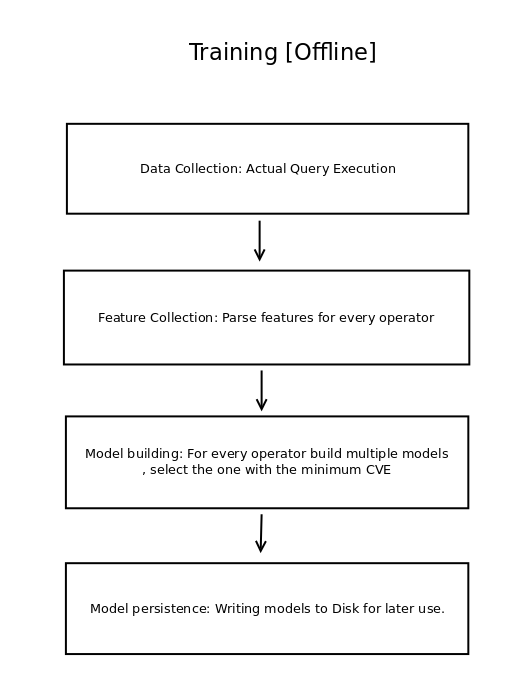
\includegraphics[scale=0.4]{training.png}

	In this section, we elaborate on the overview of the approach which consists of 2 phases. Like 
	most other machine learning approaches, the first phase is an off-line training phase and the 
	second is on-line testing phase.
	During the training phase, we construct number of different 
	models for each type of database operator. Each operator will be associated with so called 'Best-Fit' 		model which will be determined 
	based on the model selection described in next section. Later, while in testing, only this model will 		be invoked for the purpose of estimating the execution time of an operator. 
%	Since there are 			only finite number of operators and only a couple of physical implementations for them, the space 			consumption is not excessive. 

\hfill
	
	During the testing phase, we actually run the query to obtain true cardinalities. While this
	seems to contradict the whole estimation problem, right now this is required because the focus is on
	solving the modeling problem given the true cardinalities. The more practical scenario i.e., where
	we only the know the estimated cardinalities, is a much harder problem as now the models also 
	need to be Robust to the errors in cardinality estimates. 
	Once after the execution of the query, we need to extract features depending on the operator and 
	invoke the Best Fit model (which is already computed during training phase) to get an estimate. We 
	sum up costs for all the operators present in the plan tree to finally give an estimate of execution 
	time. 	


%%%%%%%%%%%%%  This can be followed by several other sections
	\section{Training}
	
	\subsection{Features}
	In this section, we describe set of possible features that we can use as input to operator level models. Features can be classified into global as well as local features. Global features are common to all operators while the local operators are specific to some operator(s). 

	\begin{center}
	\begin{tabular}{|c|c|} 
	\hline
	  Name & Description \\ \hline
	  $N_{l}$ & Number of input tuples in left child \\  \hline
	  $N_{r}$ & Number of input tuples in right child \\  \hline
	  $W_{l}$ & Tuple width of left child \\ \hline
	  $W_{r}$ & Tuple width of right child \\ \hline
	  COP & Names of child operators (Categorical) \\ \hline
	  POP & Name of parent operator(Categorical) \\ \hline
	  LOOPS & Number of loops \\ \hline
	\end{tabular}
	\\
	\vspace{.5cm}
	\textbf{Table 1: Global features}
	\end{center}
	
	
	\begin{center}
	\begin{tabular}{|c|c|c|} 
	\hline
	  Description & Operator\\ \hline
	  Levels of access in Index & IndexScan\\  \hline
	  Sort Columns & Sort\\  \hline
	  Columns involved in sort & Sort\\  \hline
	  Columns involved in Hash & Hash\\  \hline
	  Number of buckets & Hash\\  \hline
	  Number of pages read & Scan\\  \hline
	\end{tabular}
	\\
	\vspace{.5cm}
	\textbf{Table 2: Local features}
	\end{center}
	
	Please note that a) the proposed feature set should not be considered complete as it may not capture all the properties that impact execution time, we shall review these set of features from time to time as we make progress in this work.  b) More number of features 	correspond to increased training time and since the computation of Best Fit Model is exponential to the number of features, we should select as few features as possible to make the computations tractable. The task of computing which features are most important is not trivial and requires further analysis.
	
	In this primarily work, we are considering only the 2 most important features $N_{l}$ and $N_{r}$ and the models were only built on these features. Including the full feature set will enable the model to generalize further.
	
	\subsection{Model Selection}
	The relation between features and target in our case can be determined either through a) Non linear regression model b) Linear regression model with transformed features. Through our experiments we realized that Non linear regression requires much more training data than linear regression model to obtain the same accuracy. Since from SQL processing knowledge we know the possible set of functions that can relate features to execution time we instead took the approach of linear regression. Here, we have used functions that are similar to the one's defined in \cite{robustIISc}, 
	\begin{itemize}
	\item Linear: $a_{0} N_{l} + a_{1} N_{r}$ 
	\item Quadratic: $a_{0} N_{l}N_{r}$ , $a_{0} N_{l}N_{l}$ , $a_{0} N_{r}N_{r}$ \ldots
	\item Logarithmic: $a_{0} N_{l} log(N_{r}) , a_{0} N_{r} log(N_{l}) $ .. 
	\item Exponential: $a_{0} N_{l} ^ {N_{r}}$  	
	\end{itemize}	
	
	Since we don't know beforehand which function fits best without building 
	and testing, we have to explore all the possible combinations among features. 
	To illustrate the use of the functions in more details, we have plotted the curves
	with different possible functions for Quick-Sort as well as NestedLoop-Index (NL-Index) operator. For the purpose of generating curves for Quick-Sort we have used the 
	following Query template 
	
	\begin{framed}
	\begin{verbatim}
	Select * from orders
	where o_orderkey <= :varies 
	order by o_totalprice
	\end{verbatim}
	\end{framed}

%	\caption{Evaluating function $ N_{l} log(N_{l}$, this as we expected fits with very high accuracy }
\begin{center}

	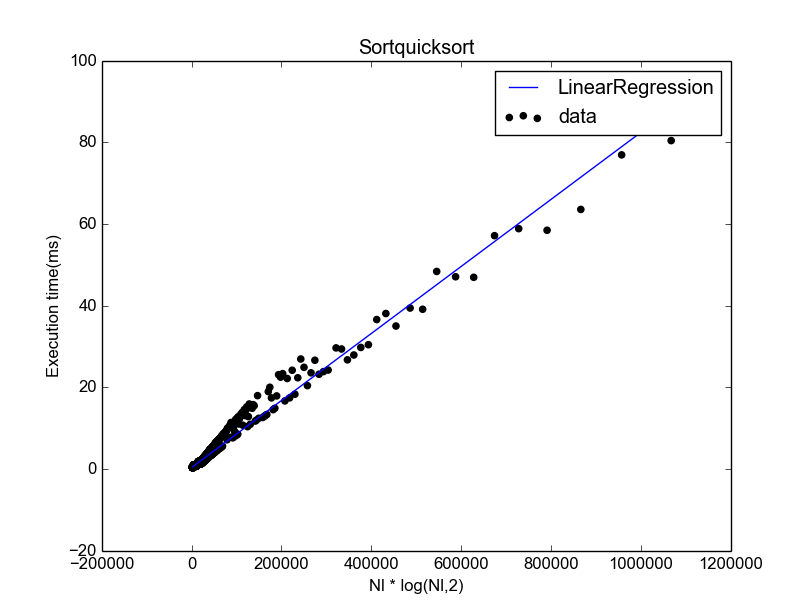
\includegraphics[scale=0.37]{Plots/quicksortnlogn.png}
	\textit{\small Evaluating $N_{l} log N_{l}$ for QuickSort}
	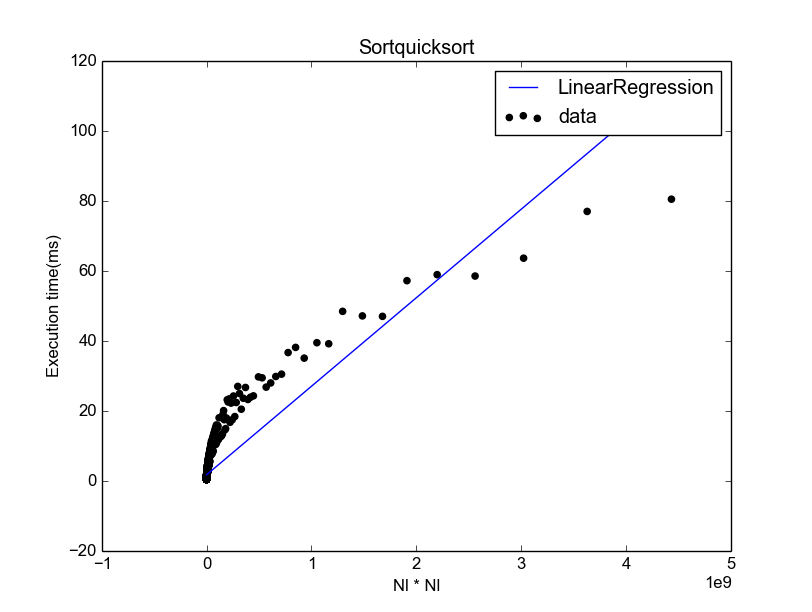
\includegraphics[scale=0.37]{Plots/quicksortnl2.png}	
	\textit{\small Evaluating $N_{l}*N_{l}$ for QuickSort}
	
\end{center}

	Unsurprisingly, logarithmic function fits better than the quadratic. 
	While in some cases (such as Quick-Sort) the appropriate function is obvious from SQL
	query processing, it does not hold for all operators. 
	For example, consider Nested-Loop join which 
	can be modeled with quadratic functions in general but when the inner relation has an 
	index 
	the same model produces estimates estimates which are 
	"off" by orders of magnitude because now with the index on inner tables joins can be done much faster than before. Unless this is accounted separately in the learning model, it degrades the overall model for NestedLoop. This also explains why learning need to be done at implementation level and not at operator or plan level. 
	
Now we illustrate the same in the following example by taking exploratory approach to determine the best fit function for the NL-Index operator.
	As in the case of Quick-Sort we have used the following query template to generate the required
	data.
	
	\begin{framed}
	\begin{verbatim}
	select * from lineitem,orders
	where l_orderkey = o_orderkey 
		  and l_orderkey<= : varies;
	\end{verbatim}
	\end{framed}
	
	
	\begin{center}
	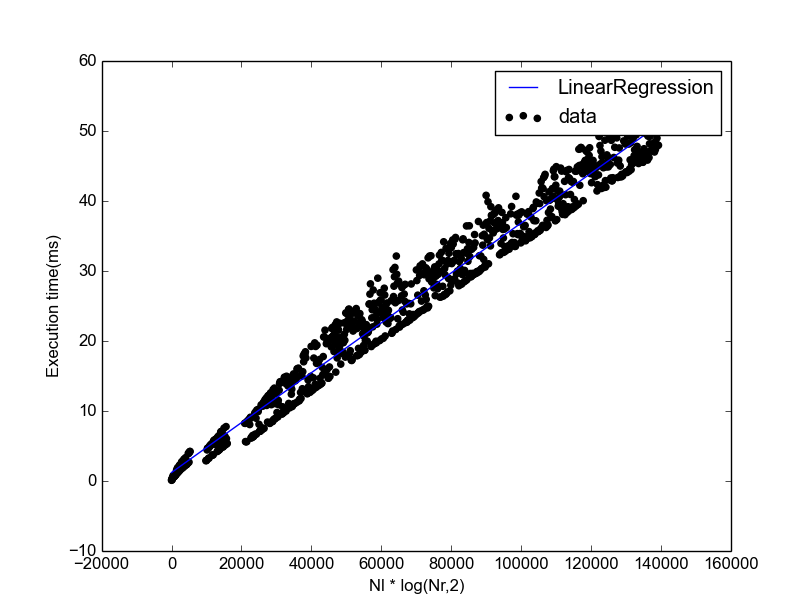
\includegraphics[scale=0.37]{Plots/nil-nlnrlog2.png}	
	\textit{\small Evaluating $N_{l} log N_{r}$ for NL-Index}
	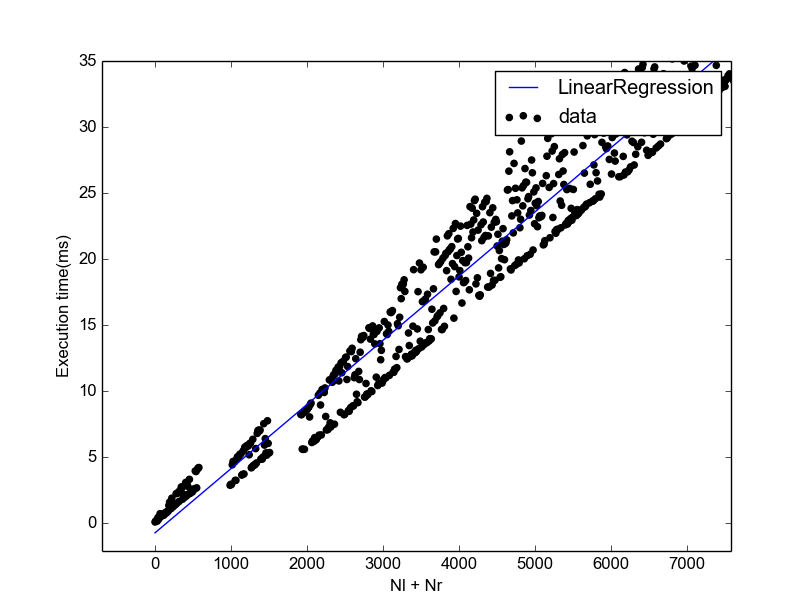
\includegraphics[scale=0.37]{Plots/nil-nl+nr.png}	
	\textit{\small Evaluating $N_{l} + N_{r}$ for NL-Index}
	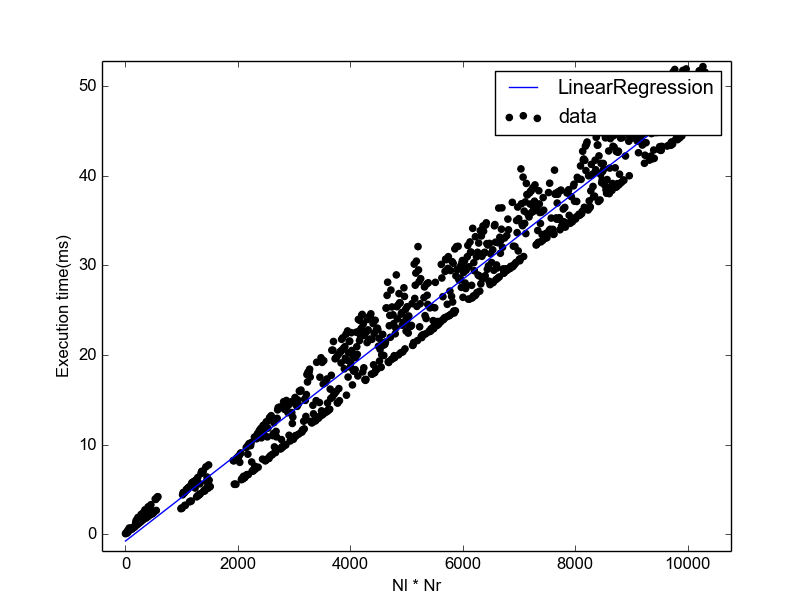
\includegraphics[scale=0.37]{Plots/nil-nlnr.png}	
	\textit{\small Evaluating $N_{l} * N_{r}$ for Nl-Index}
	\end{center}
	
	Out of the above 3 functions, $N_{l} log(N_{r})$ fits data better than alternative functions which makes it the Best Fit Model for Nl-Index operator, the other models are discarded. 	
	\subsection{Best Fit Model}	
	Best fit model $M_{O}$ for an Operator $O$ is the model which has the minimum estimation error 
	for the set of training queries. The estimation error is computed as follows,
	
	\begin{center}
	$\dfrac{1}{n} \sum\limits_{i=1}^n \left| Actual_{i} - Estimated_{i} \right|$
	\end{center}
	
	\section{Preliminary Experiments}
	\subsection{Setup}
	Our experimental study uses TPC-H decision support benchmark \cite{TPCH} on the top of 
	PostgresSQL. The details are as follows, 

	\begin{itemize}
	\item Database Management System : Default PostgreSQL 9.4. Currently, we have not tuned 
	any Postgres parameters. %which might improve its cost-model performance.
	\item Data sets and workload: We created 1GB TPC-H database
	according to the specification. In this work, we are limiting ourselves to in-memory 
	environment. The primary key indices as indicated
	in the TPC-H specification were created for both databases. We have excluded Query 1,21  
	because the execution plans generated are not compliant with our current tree based 
	model, and Queries 15 as it creates a view which is 
	not yet	supported in our work. This resulted in 19 out of 22 TPC-H queries being used 
	for training. We've used TPC-H qgen tool to generate 10 instances of each of the 19 
	queries, resulting in a total of 190 queries.
	
	\item Hardware: The queries were executed on a machine
	with 8GB RAM running Ubuntu. buffer pool size was set to 1GB. All queries were executed 
	sequentially with cold start (i.e., OS buffers flushed before the start of each query).
	
	\item Statistical Models: For evaluating the best-fit model we have used linear regression and Support Vector Regression \cite{sckit}
	
	
	\end{itemize}		
	
	\subsection{Prediction with Optimizer cost models}		
	We start with the results showing that Optimize estimates are a poor indication of the real
	execution time. For this purpose, we have taken 19 of 22 queries (To make a fair comparison with 
	our approach we've excluded the 3 templates for the reason stated earlier). The values collected are averaged over 5 runs.
	\begin{center}
	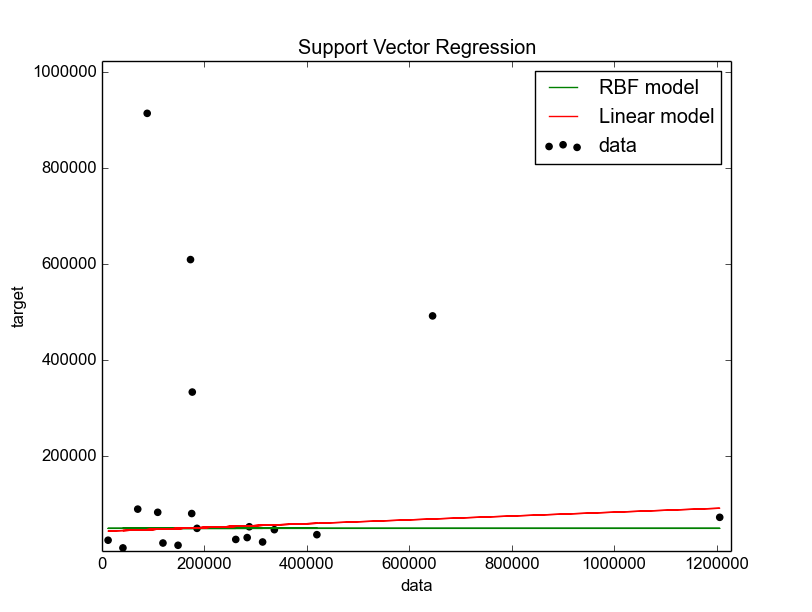
\includegraphics[scale=0.45]{optcost.png}
	\\
	\vspace{0.5cm}
	\textbf{Figure 1 : Optimizer estimates can incur significant errors}
	\end{center}
	\setcounter{figure}{1}
	
	Observe that lower left and upper left data points correspond to same
	optimizer cost but differ significantly in the actual execution time.
	We've plotted the linear regression line resulting from fitting these points 
	using linear least-squares regression 
	(which can be seen as an error-minimizing mapping of the
	optimizer-estimated cost (which is not measured in ms) to CPU-
	time). As we can see, even for the mapping chosen to minimize
	the overall error, there are significant differences between the estimated CPU cost 
	and real CPU time for many queries. Similar
	observations have been made in other works as well \cite{MSR,ICDE2012}

	Note that while the final estimate made by the optimizer may not be an accurate reflection of
	real execution time, the estimates provided at a finer level (i.e., plan level, operator level etc.) 
	are quite useful. In the next section, we show how we can use optimizer estimates at operator level 
	and produce an estimate for overall execution time.
	
	\subsection{Operator level modeling}
	\begin{figure*}[!t]
	  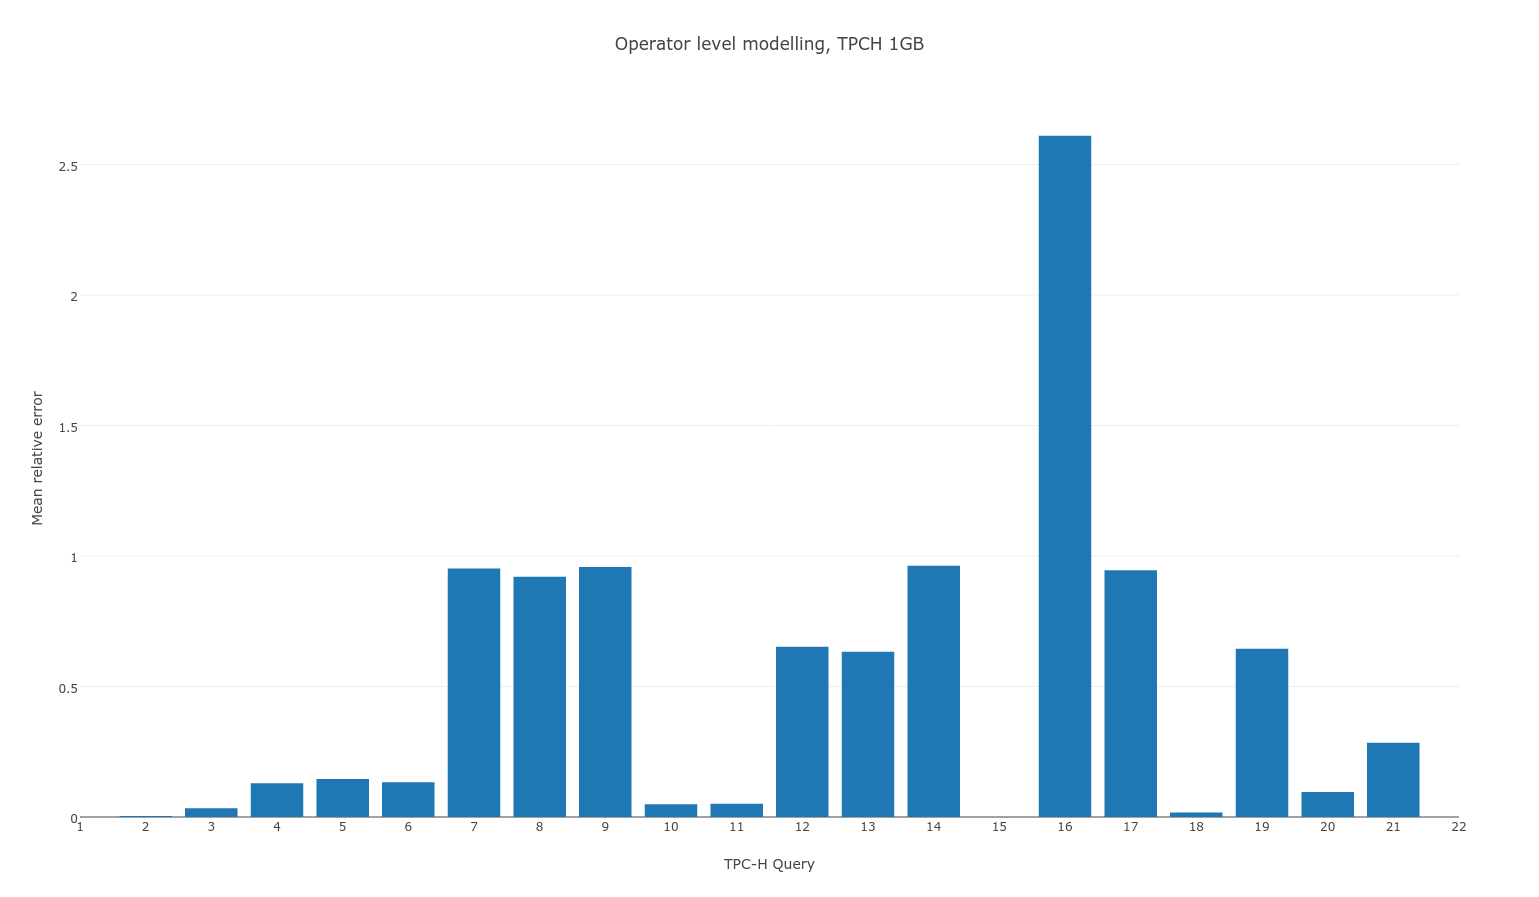
\includegraphics[width=\textwidth]{tpch-1gbres.png}
	  \caption{{Operator-level modeling ,Errors by Template (1GB)}}
	\end{figure*}
	
	To ensure that the trained model is not over-fitting the data, we have generated training and testing queries do not contain identical instances of same query (i.e, same query with same selectivities is not allowed). 
	
	\begin{center}
	\begin{tabular}{|c|c|c|c|} 
	\hline
	  Model & Min RE & Max RE & Mean RE \\ 	 \hline
	 Optimizer & 0.032  & 47.68 & 8.33 \\ \hline
	 Our model & 0.003 & 2.61 & 0.53 \\ \hline
	\end{tabular}
	\\
	\vspace{.5cm}
	\textbf{Table 3: Relative error(RE) for TPC-H, 1GB}
	\end{center}

	The benefits of operator level modeling can be clearly
	seen here. The optimizer cost model has a mean
	MRE of 8.33 i.e., on an average it predicts within 800\%
	actual execution time. Experiments on TPC-H queries
	shows that optimizer cost estimate can degrade to as
	much as 4700\%.
	In Figure 2, we have shown the error obtained
	for individual queries, our model produced estimates
	that deviate by at-most 261\% and on-an average were
	within 48\% of actual execution time. By using additional 
	features we believe we can further bring this
	down. To evaluate why certain queries are doing bad,
	we dug into the plan tree and found that for the operators 
	HashJoin, Materalize, BitmapHeapScan and
	NestedLoop the model is producing estimates with
	high MRE’s.
	
%	Give a background about Static and dynamic workload.  
%	do experiments at 2 stages
%	1. Act vs Act
%	2. Est vs Est(Bias towards estimated cardinalities)
%	For each type of above scenario, do testing for tpc-h queries 
%	(tpc-ds in future)
%	At different scales to see the model's ability to predict.
%	For midterm you should be having result for 1 as well as 10 GB.
%	For each above dataset, 
%	Results should convey L1 (MRE) as well as queries that are within 
%	[0-0.5] [0.5-1] [1-1.5] 

	\section {Related work}
	Query-plan-level predictions have recently been studied \cite{ganapathi}. In \cite{ganapathi},
	authors consider plan-level query performance prediction for the
	following \textit{static} query workloads: the TPC-DS query benchmark
	and a query workload obtained from a customer database. They
	report that they can predict individual query execution times within
	20\% of the actual time for 85\% of their test queries.	However their approach produces
	poor estimates for queries which are \textit{different} from training queries. The ability to 
	adapt to dynamic workload is crucial for the cost model to continuously adapt the changes in the
	underlying databases and queries.
	
	In \cite{ICDE2012, MSR} authors proposed an approach which learns at a finer granularity than 
	at plan level. They use statistical models such as SVM and Linear regression to learn the behavior of 
	every operator. They have shown by that learning at this level, the model can now recognize queries 		which can differ largely from the queries seen during training. They have only considered 14 out of 		22 templates and claimed that they were able to obtain 41\% i.e., an MRE of 0.41. We are different 			from their approach in 2 ways a) we consider learning at \textit{implementation level} i.e, for the operator \textit{sort}, to implement it optimizer has a choice among multiple sorting methods such as quick sort ,merge sort top-N heapsort and external sort etc. No previous learning based approach distinguishes the implementation methods of an operator which is clearly incorrect because there's a substantial difference between resource consumptions of quick-sort and external sort as the former is CPU intensive (consumes relatively less time) and while the latter is IO intensive (consumes much more time). b) we consider multiple learning models for every implementation and select the one which fits the best. This approach is often used when the relation between features and target is unclear. 
	
	In \cite{analytical}, authors have done an analytical cost modeling where in they compute CPU and IO time individually by obtaining the number of operations performed and number of pages(sequential \& random) accessed respectively. They have also proposed a calibration phase where the cost model can account for the hardware changes which is absent in default Postgres model. In previous report by Pankhuri, methods are provided to compute cost for reading random page which was ambiguous the work\cite{analytical}. While this kind of approach seems natural, interactions among query operators (such as pipelining) 
	
	Finally, there has also been work on query progress indicators \cite{progress}. Query progress indicators provide estimations for the completion degrees of running queries. Such studies assume that the work
	done by individual query operators are transparent, i.e., externally
	visible. While these studies are also related to query execution performance,
	they do not provide predictions for the execution time of
	queries.
	
	\section{Conclusions and Future Work}
	In this work, we have presented learning based approach at a finer granularity than whats proposed earlier in the literature. By learning at implementation level we have shown that the model can generalize to the queries which are unseen during the training.
	There remains a lot of work to be done. The feature set need to be extended to include operator specific features and parameters which can capture the effects of pipeline. The resulting model will be more accurate and also will be able to generalize to different queries and database scales.
	
%	We have assumed that we are getting true cardinalities, where in the practical scenario they will often have magnitude of errors. If we train the model with optimizers estimates instead of true cardinalities, the model to certain extent can have a bias towards estimation errors. On the other hand, we can have partial executions 
	

	
	\begin{thebibliography}{9}
			\bibitem{analytical}
	Wu, Wentao, et al. "Predicting query execution time: Are optimizer cost models really unusable?." ICDE 2013.

	\bibitem{concurrent}
	Wu, Wentao, et al. "Towards predicting query execution time for concurrent and dynamic database workloads." Proceedings of the VLDB Endowment (2013)


	\bibitem{ICDE2012}
	Akdere, Mert, et al. "Learning-based query performance modeling and prediction." ICDE 2012.

	\bibitem{MSR}
	Li, Jiexing, et al. "Robust estimation of resource consumption for sql queries using statistical techniques." Proceedings of the VLDB Endowment (2012)
	

	\bibitem{sckit}
	Scikit-learn: Machine Learning in Python, Pedregosa et al., JMLR 12, pp. 2825-2830, 2011.


	\bibitem{activeSLA}
	Xiong, Pengcheng, et al. "ActiveSLA: a profit-oriented admission control framework for database-as-a-service providers." Proceedings of the 2nd ACM Symposium on Cloud Computing. ACM, 2011.	

	\bibitem{ganapathi} 
	Ganapathi, Archana, et al. "Predicting multiple metrics for queries: Better decisions enabled by machine learning." ICDE 2009.
	
     
    \bibitem{adaptive} 
     Guirguis, Shenoda, et al. "Adaptive scheduling of web transactions." ICDE 2009.
	
	\bibitem{robustIISc}
	Harish, D., Pooja N. Darera, and Jayant R. Haritsa. "Identifying robust plans through plan diagram reduction." Proceedings of the VLDB Endowment (2008)
	
	\bibitem{TPCDS}
	R. Othayoth and M. Poess, The making of TPC-DS, Proceedings VLDB Endowment (2006).

	\bibitem{progress}
	Chaudhuri, Surajit, Vivek Narasayya, and Ravishankar Ramamurthy. "Estimating progress of execution for SQL queries." Proceedings of the 2004 ACM SIGMOD international conference on Management of data. ACM, 2004.
	
	\bibitem{nestedloops}
	DeWitt, David J., Jeffrey F. Naughton, and Joseph Burger. "Nested loops revisited." Parallel and Distributed Information Systems, 1993., Proceedings of the Second International Conference on. IEEE, 1993.
	
	\bibitem{TPCH}
	TPC-H benchmark specification, http://www.tpc.org/tpch/

	
	\end{thebibliography}
	\end{multicols}
\end{document}
